


\section{intro}

\begin{frame}{The Internet}
    \begin{itemize}
    \item Perhaps the most successful computer application ever
    \item Can you name a computer program that doesn't use the internet?
    \end{itemize}
\end{frame}

\begin{frame}{}
\begin{center}
\includegraphics[width=0.8\pagewidth]{../network/internet_users.png}
\end{center}
\end{frame}

\begin{frame}{}
\begin{center}
\includegraphics[width=0.8\pagewidth]{../network/internet_reasons.png}
\end{center}
\end{frame}

\begin{frame}{}
\begin{center}
\includegraphics[width=0.8\pagewidth]{../network/internet_data.png}
\end{center}
\end{frame}


\section{sockets}

\begin{frame}{sockets is the de-facto API for networking}
    \begin{itemize}
    \item open connection then \ldots
        \begin{itemize}
        \item read+write just like a terminal file
        \end{itemize}
    \vspace{.5cm}
    \item doesn't look like individual messages
    \item ``connection abstraction''
    \end{itemize}
\end{frame}

\section{mailbox model}

\usetikzlibrary{arrows.meta,shapes.symbols,shapes.multipart}

\begin{frame}{mailbox model}
    \begin{itemize}
    \item \textit{mailbox} abstraction: send/receive messages
    \end{itemize}
    \begin{tikzpicture}
    \tikzset{
        >=Latex,
        comp box/.style={draw, thick, align=center, minimum width=1.5cm,minimum height=3cm},
        explain box/.style={draw=red,very thick, align=left},
        msg/.style={font=\small},
        cmd/.style={font=\small},
    }
        \node[comp box] (machine A) at (-6.5, 0) {machine \\ A};
        \node[draw,cloud,line width=1pt,minimum width=4cm,minimum height=1cm,aspect=3,
                alt=<2>{red,thick}] (network) at (0,0) {the network};
        \node[comp box] (machine B) at (6.5, 0) {machine \\ B};
        \draw[very thick,->] (machine A) -- (network) 
            node[midway,above,msg] {B: ``Hello''}
            node[pos=0.0,below right,cmd] {Send(B, ``Hello'')};
        \draw[very thick,<-] (machine B) -- (network) 
            node[midway,above,msg] {B: ``Hello''}
            node[pos=0.0,below left,cmd] {Recv() = ``Hello''};
        % FIXME: hilite network: knows how to get message to particular place
            % note/show buffering at A/B
        \begin{visibleenv}<2>
            \node[explain box,anchor=north] at ([yshift=-.25cm]network.south) {
                network knows how to get message to B
            };
        \end{visibleenv}
        \begin{visibleenv}<3->
            \node[anchor=south,draw,rectangle,rectangle split,rectangle split parts=5,rectangle split horizontal, inner sep=0.25mm] at ([yshift=.1cm]machine A.south) {
                ~~~
            };
        \end{visibleenv}
        \begin{visibleenv}<3>
            \node[explain box,anchor=north] at ([yshift=-.25cm]network.south) {
                queue of messages \\
                from sending program \\
                waiting to be sent
            };
        \end{visibleenv}
        \begin{visibleenv}<4->
            \node[anchor=south,draw,rectangle,rectangle split,rectangle split parts=5,rectangle split horizontal,inner sep=0.25mm] at ([yshift=.1cm]machine B.south) {
                ~~~
            };
        \end{visibleenv}
        \begin{visibleenv}<4>
            \node[explain box,anchor=north] at ([yshift=-.25cm]network.south) {
                queue of messages \\
                not yet received by \\
                receiving program
            };
        \end{visibleenv}
    \end{tikzpicture}
\end{frame}

\begin{frame}{connections over mailboxes}
    \begin{itemize}
    \item real Internet: mailbox-style communication
        \begin{itemize}
        \item send packets to particular mailboxes
        \item no gaurentee on order, when received
        \end{itemize}
    \item sockets implemented on top of this
    \end{itemize}
\end{frame}


 % FIXME: wrong place?

\section{review: connection abstraction}

\input{../network/connection-model}

\section{layers preview}
\begin{frame}<1>[fragile,label=layerOverview]{networking layers}
\begin{tabular}{|l|l|p{6cm}|} \hline
application           & HTTP, SSH, SMTP, \ldots & {application-defined meanings}                                     \\ \hline
\myemph<6>{transport} & TCP, UDP, \ldots        & {reach correct program,\linebreak \myemph<2>{reliability/streams}} \\ \hline
\myemph<5>{network}   & IPv4, IPv6              & {reach correct machine}\linebreak(across networks)                 \\ \hline
\myemph<4>{link}      & Ethernet, Wi-Fi, \ldots & {coordinate shared wire/radio}                                     \\ \hline
physical              & Ethernet, Wi-Fi, \ldots & encode bits for wire/radio                                         \\ \hline
\end{tabular}
\end{frame}

\begin{frame}<1>[fragile,label=layerMsgNames]{layers terminology}
\begin{tabular}{|l|p{6cm}|l|} \hline
application & {application-defined meanings} & ~\\ \hline
transport & {reach correct program,\linebreak reliablity/streams} & segments/datagrams \\ \hline
network & {reach correct machine}\linebreak(across networks) & packets \\ \hline
link & {coordinate shared wire/radio} & frames \\ \hline
physical & encode bits for wire/radio & ~ \\ \hline
\end{tabular}
\end{frame}


\subsection{layer wrapping}
\begin{frame}{layer wrapping}
    \begin{itemize}
    \item upper layers usually implemented using lower layers
    \vspace{.5cm}
    \item example: implement reliable + large messages (transport layer) \\
        by sending multiple unreliable messages across networks (network layer)
    \item example: implement reaching machine across networks (network layer) \\
        by sending multiple messages on local networks (link layer)
    \end{itemize}
\end{frame}


\section{handling network failures}
\againframe<2>{layerOverview}

\begin{frame}{reality: you don't own the network!}
    \begin{itemize}
    \item the internet is a series of connected networks
    \item packets traverse routers within and between networks
    \item those networks provide ``best-effort'' service
    \end{itemize}
    \begin{center}
        \includegraphics[width=0.4\pagewidth]{../network/network-of-network}
    \end{center}
\end{frame}


\begin{frame}<1>[label=netFailTypes]{network limitations/failures}
    \begin{itemize}
    \item \myemph<2>{messages lost}
    \item \myemph<3>{messages delayed/reordered}
    \item \myemph<4>{messages limited in size}
    \item \myemph<5>{messages corrupted}
    \end{itemize}
\end{frame}



\subsection{acknowledgments}
\againframe<2>{netFailTypes}
\usetikzlibrary{arrows.meta,shapes.misc,decorations.pathreplacing}

\begin{frame}{dealing with network message lost}
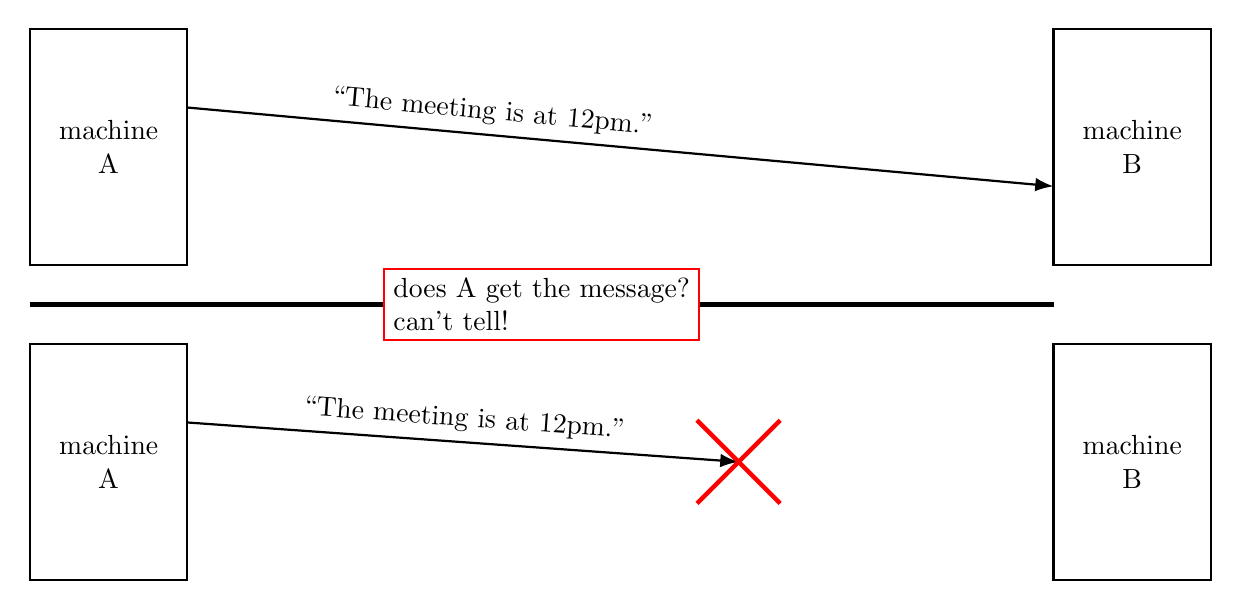
\begin{tikzpicture}
\tikzset{
    box/.style={draw,thick,minimum width=2cm},
    message/.style={draw,thick,-Latex},
    failure/.style={draw,ultra thick,red,cross out,minimum width=1cm,minimum height=1cm},
}
\begin{scope}
\draw[box] (0, 0) rectangle ++(2, -3) 
    node[midway,align=center] {machine\\ A};
\draw[box] (13, 0) rectangle ++(2, -3) 
    node[midway,align=center] {machine\\B};
\draw[message] (2, -1) -- (13, -2) node[pos=0.35, above, sloped] {``The meeting is at 12pm.''};
\end{scope}
\draw[ultra thick] (0, -3.5) -- ++ (13,0);
\begin{scope}[yshift=-4cm]
\draw[box] (0, 0) rectangle ++(2, -3) 
    node[midway,align=center] {machine\\A};
\draw[box] (13, 0) rectangle ++(2, -3) 
    node[midway,align=center] {machine\\B};
\draw[message] (2, -1) -- (9, -1.5) 
    node[pos=0.5,above,sloped] {``The meeting is at 12pm.''}
    node[failure] {};
\end{scope}
\node[draw=red,thick,fill=white,align=left] at (6.5, -3.5) {
    does A get the message? \\
    can't tell!
};
\end{tikzpicture}
\end{frame}

\begin{frame}{handling lost message: acknowledgements}
\begin{tikzpicture}
\tikzset{
    box/.style={thick},
    message/.style={draw,thick,-Latex},
    failure/.style={draw,ultra thick,red,cross out,minimum width=1cm,minimum height=1cm},
}
\begin{scope}
\draw[box] (0, 0) rectangle ++(2, -8) 
    node[midway,align=center] {machine\\A};
\draw[box] (13, 0) rectangle ++(2, -8) 
    node[midway,align=center] {machine\\B};
\draw[message] (2, -0.5) -- (13, -1) node[pos=0.35, above, sloped] {``The meeting is at 12pm.''};
\draw[message] (13, -1.5) -- (2, -2) node[pos=0.25, sloped,below] {Got it!};
\end{scope}
\end{tikzpicture}
\end{frame}

\begin{frame}{handling lost message}
\begin{tikzpicture}
\tikzset{
    box/.style={thick},
    message/.style={draw,thick,-Latex},
    failure/.style={draw,ultra thick,red,cross out,minimum width=1cm,minimum height=1cm},
}
\draw[box] (0, 0) rectangle ++(2, -8) 
    node[midway,align=center] {machine\\A};
\draw[box] (13, 0) rectangle ++(2, -8) 
    node[midway,align=center] {machine\\B};
%\draw[message] (2, -0.5) -- (13, -1) node[pos=0.35, above, sloped] {``The meeting is at 12pm.''};
\draw[message] (2, -0.5) -- (9, -1) 
    node[pos=0.5,above,sloped] {``The meeting is at 12pm.''}
    node[failure] {};
\begin{visibleenv}<2->
\draw[decorate,decoration={brace}] (2.1, -1) -- (2.1, -3) 
    node[midway,right,align=left] {
        ``timeout'' \\
        A doesn't get reply \\
        after waiting too long
    };
\end{visibleenv}
\begin{visibleenv}<3->
\draw[message] (2, -4) -- (13, -5) node[pos=0.35, above, sloped] {``The meeting is at 12pm.''};
\draw[message] (13, -5.5) -- (2, -6) node[pos=0.5, sloped,below] {Got it!};
\end{visibleenv}
\end{tikzpicture}
\end{frame}

\begin{frame}{lost acknowledgements}
\begin{tikzpicture}
\tikzset{
    box/.style={thick},
    message/.style={draw,thick,-Latex},
    failure/.style={draw,ultra thick,red,cross out,minimum width=1cm,minimum height=1cm},
}
\draw[box] (0, 0) rectangle ++(2, -8) 
    node[midway,align=center] {machine\\A};
\draw[box] (13, 0) rectangle ++(2, -8) 
    node[midway,align=center] {machine\\B};
\draw[message] (2, -0.5) -- (13, -1) node[pos=0.35, above, sloped] {``The meeting is at 12pm.''};
\draw[message] (13, -1.5) -- (6.5, -1.75) node[pos=0.5, sloped,below] {Got it!}
    node[failure] {};
\begin{visibleenv}<3->
\draw[message] (2, -3.5) -- (13, -4) node[pos=0.35, above, sloped] {``The meeting is at 12pm.''};
\draw[message] (13, -4.5) -- (2, -5) node[pos=0.5, sloped,below] {Got it!};
\end{visibleenv}
\begin{visibleenv}<2>
\node[draw=red,thick,fill=white,align=left] at (6.5, -6.5) {
    A's going to need to resend this message! \\
    Can't tell it really was received!
};
\end{visibleenv}
\begin{visibleenv}<3>
\node[draw=red,thick,fill=white,align=left] at (6.5, -6.5) {
    B needs to handle receiving message twice! \\
    Sockets: you only get a copy of the data once.
};
\end{visibleenv}
\end{tikzpicture}
\end{frame}


\begin{frame}{delayed acknowledgements}
\begin{tikzpicture}
\tikzset{
    box/.style={thick},
    message/.style={draw,thick,-Latex},
    failure/.style={draw,ultra thick,red,cross out,minimum width=1cm,minimum height=1cm},
}
\draw[box] (0, 0) rectangle ++(2, -8) 
    node[midway,align=center] {machine\\A};
\draw[box] (13, 0) rectangle ++(2, -8) 
    node[midway,align=center] {machine\\B};
\draw[message] (2, -0.5) -- (13, -1) node[pos=0.35, above, sloped] {``The meeting is at 12pm.''};
\draw[message] (13, -1.5) -- (2, -5) node[pos=0.25, sloped,below] {Got it!};
\draw[decorate,decoration={brace}] (2.1, -1) -- (2.1, -3) 
    node[midway,right,align=left] {
        ``timeout''
    };
\begin{visibleenv}<3->
\draw[message] (2, -3.5) -- (13, -4) node[pos=0.35, above, sloped] {``The meeting is at 12pm.''};
\draw[message] (13, -4.5) -- (2, -6) node[pos=0.5, sloped,below] {Got it!};
\end{visibleenv}
\begin{visibleenv}<3>
\node[draw=red,thick,fill=white,align=left] at (8, -6.5) {
    B can't tell that first acknowledgment wasn't lost
};
\end{visibleenv}
\end{tikzpicture}
\end{frame}

\subsubsection{exercise: lost acks}
\begin{frame}{exercise: lost acknowledgement}
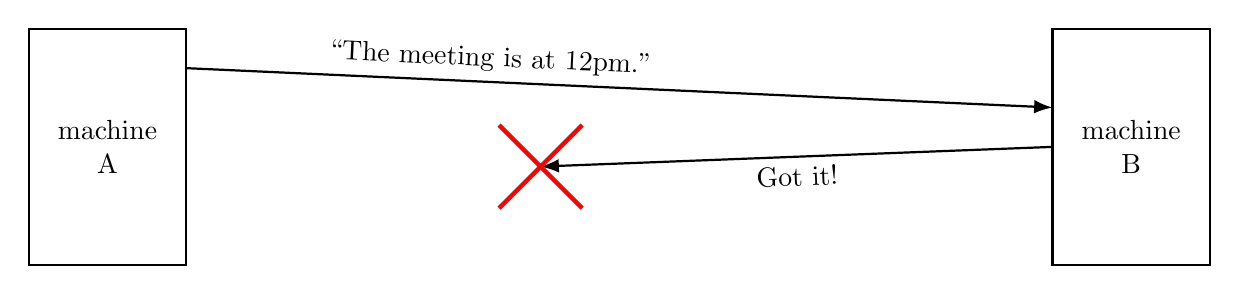
\begin{tikzpicture}
\tikzset{
    box/.style={thick},
    message/.style={draw,thick,-Latex},
    failure/.style={draw,ultra thick,red,cross out,minimum width=1cm,minimum height=1cm},
}
\draw[box] (0, 0) rectangle ++(2, -3) 
    node[midway,align=center] {machine\\A};
\draw[box] (13, 0) rectangle ++(2, -3) 
    node[midway,align=center] {machine\\B};
\draw[message] (2, -0.5) -- (13, -1) node[pos=0.35, above, sloped] {``The meeting is at 12pm.''};
\draw[message] (13, -1.5) -- (6.5, -1.75) node[pos=0.5, sloped,below] {Got it!}
    node[failure] {};
\end{tikzpicture}
exercise: how to fix this?
\begin{tabular}{ll}
A. & machine A needs to send ``Got `got it!' '' \\
B. & machine B should resend ``Got it!'' on its own \\
C. & machine A should resend the original message on its own \\
D. & none of these \\
\end{tabular}
\end{frame}

\begin{frame}<0>[label=lostAckExExplain]{answers}
\begin{itemize}
\item send ``Got `got it!' ''?
    \begin{itemize}
    \item same problem: Now send `Got Got Got it'?
    \end{itemize}
\item resend ``Got it!'' own its own?
    \begin{itemize}
    \item how many times? --- B doesn't have that info
    \end{itemize}
\item resend original message?
    \begin{itemize}
    \item yes!
    \item as far as machine A can be, \textit{exact same situation} as losing original message
    \end{itemize}
\end{itemize}
\end{frame}

\iftoggle{heldback}{}{
    \againframe<1>{lostAckExExplain}
}


\subsubsection{solution: lost acks}
\iftoggle{heldback}{}{\input{../network/fail-lost-lost-ack-explain}}
\subsubsection{delayed acks}
\againframe<3>{netFailTypes}

\begin{frame}{delayed message}
\begin{tikzpicture}
\tikzset{
    box/.style={thick},
    message/.style={draw,thick,-Latex},
    failure/.style={draw,ultra thick,red,cross out,minimum width=1cm,minimum height=1cm},
}
\draw[box] (0, 0) rectangle ++(2, -8) 
    node[midway,align=center] {machine\\A};
\draw[box] (13, 0) rectangle ++(2, -8) 
    node[midway,align=center] {machine\\B};
\draw[message] (2, -0.5) -- (13, -4.5) node[pos=0.35, above, sloped] {``The meeting is at 12pm.''};
\draw[message] (13, -4.5) -- (2, -5) node[pos=0.25, sloped,below] {Got it!};
\draw[decorate,decoration={brace}] (2.1, -1) -- (2.1, -3) 
    node[midway,right,align=left] {
        ``timeout''
    };
\begin{visibleenv}<3->
\draw[message] (2, -3.5) -- (13, -5) node[pos=0.35, above, sloped] {``The meeting is at 12pm.''};
\draw[message] (13, -5.5) -- (2, -6) node[pos=0.5, sloped,below] {Got it!};
\end{visibleenv}
\begin{visibleenv}<3>
\node[draw=red,thick,fill=white,align=left] at (8, -7) {
    B resends, can't tell message is just slow
};
\end{visibleenv}
\end{tikzpicture}
\end{frame}


\begin{frame}{delayed acknowledgements}
\begin{tikzpicture}
\tikzset{
    box/.style={thick},
    message/.style={draw,thick,-Latex},
    failure/.style={draw,ultra thick,red,cross out,minimum width=1cm,minimum height=1cm},
}
\draw[box] (0, 0) rectangle ++(2, -8) 
    node[midway,align=center] {machine\\A};
\draw[box] (13, 0) rectangle ++(2, -8) 
    node[midway,align=center] {machine\\B};
\draw[message] (2, -0.5) -- (13, -1) node[pos=0.35, above, sloped] {``The meeting is at 12pm.''};
\draw[message] (13, -1.5) -- (2, -5) node[pos=0.25, sloped,below] {Got it!};
\draw[decorate,decoration={brace}] (2.1, -1) -- (2.1, -3) 
    node[midway,right,align=left] {
        ``timeout''
    };
\begin{visibleenv}<3->
\draw[message] (2, -3.5) -- (13, -4) node[pos=0.35, above, sloped] {``The meeting is at 12pm.''};
\draw[message] (13, -4.5) -- (2, -6) node[pos=0.5, sloped,below] {Got it!};
\end{visibleenv}
\begin{visibleenv}<3>
\node[draw=red,thick,fill=white,align=left] at (8, -6.5) {
    B can't tell that first acknowledgment wasn't lost
};
\end{visibleenv}
\end{tikzpicture}
\end{frame}



\subsection{splitting into multiple}
\againframe<4>{netFailTypes}
\input{../network/fail-split}

    % FIXME: exercise
        % acknowledge only last
        % partial acknowledgments

\subsection{checksums}
\againframe<5>{netFailTypes}
\begin{frame}{message corrupted}
\begin{itemize}
\item corruption: e.g., a bit flip
	\begin{itemize}
	\item sent: \texttt{I LIKE CATS} (\texttt{49204C494B452043415453})
	\item recv: \texttt{I LIKE BATS} (\texttt{49204C494B4520\myemph{42}415453})
	\end{itemize}
\item instead of sending ``message'', send ``message'' + checksum
	\begin{itemize}
	\item checksum is some calculation using the original message
	\item ex: checksum(\texttt{I LIKE CATS}) = 0xD9
	\item send \texttt{49204C494B452043415453\myemph{D9}}
	\end{itemize}
% \vspace{.5cm}
% \item say Hash(``message'') = 0xABCDEF12
% \item then send ``0xABCDEF12,message''
\vspace{.5cm}
\item receiver then also computes the checksum with the same data
	\begin{itemize}
	\item if matches: keep the message
	\item if does not match: pretend like the message was lost (i.e., drop the message)
	\end{itemize}
% \item pretend message lost if does not match
\end{itemize}
\end{frame}

% \begin{frame}{``checksum''}
% \begin{itemize}
% \item these hashes commonly called ``checksums''
% \item in UDP/TCP, hash function: treat bytes of messages as array of integers; then add integers together
% \end{itemize}
% \end{frame}

    % FIXME: exercise:

\subsection{aside: going faster}
\begin{frame}{going faster}
    \begin{itemize}
    \item so far: send one message, wait for acknowledgment
    \vspace{.5cm}
    \item very slow!
    \item instead, can send a bunch of parts and get them acknowledged together
    % \item need to do \textit{congestion control} to avoid overloading network
    \end{itemize}
\end{frame}

\usetikzlibrary{arrows.meta,decorations.pathreplacing,shapes.misc}

\begin{frame}{transmission window (ex: size 4)}
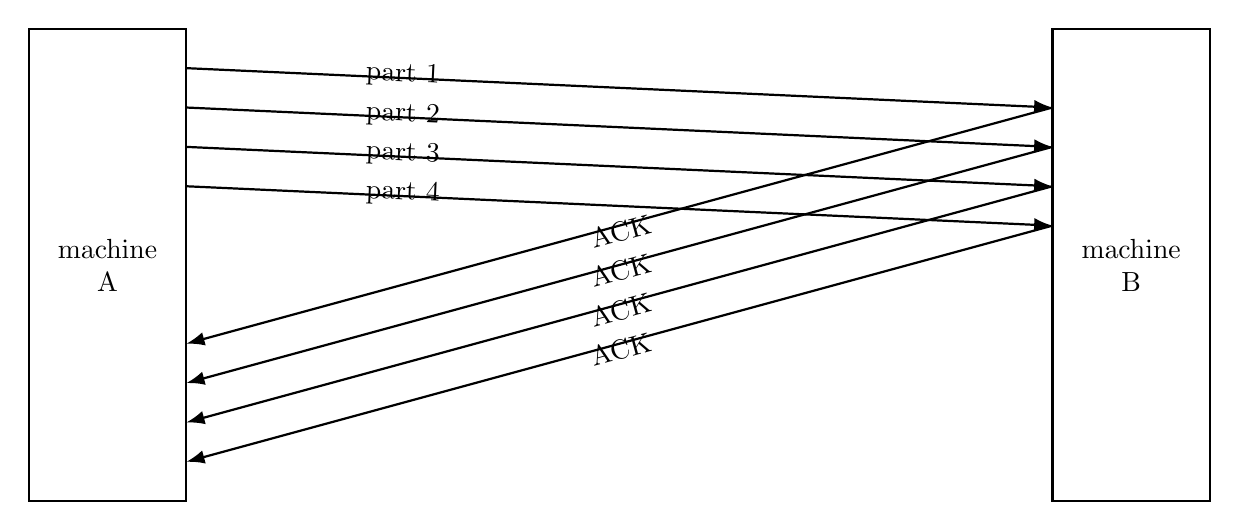
\begin{tikzpicture}
\tikzset{
    box/.style={thick},
    message/.style={draw,thick,-Latex},
    failure/.style={draw,ultra thick,red,cross out,minimum width=1cm,minimum height=1cm},
}
\begin{scope}
\draw[box] (0, 0) rectangle ++(2, -6)
    node[midway,align=center] {machine\\A};
\draw[box] (13, 0) rectangle ++(2, -6)
    node[midway,align=center] {machine\\B};
\draw[message] (2, -0.5) -- (13, -1.0) node[pos=0.25, above=-7pt, sloped] {part 1};
\draw[message] (2, -1.0) -- (13, -1.5) node[pos=0.25, above=-7pt, sloped] {part 2};
\draw[message] (2, -1.5) -- (13, -2.0) node[pos=0.25, above=-7pt, sloped] {part 3};
\draw[message] (2, -2.0) -- (13, -2.5) node[pos=0.25, above=-7pt, sloped] {part 4};
\draw[message] (13, -1.0) -- (2, -4.0) node[pos=0.5, sloped, below=-5pt] {ACK};
\draw[message] (13, -1.5) -- (2, -4.5) node[pos=0.5, sloped, below=-5pt] {ACK};
\draw[message] (13, -2.0) -- (2, -5.0) node[pos=0.5, sloped, below=-5pt] {ACK};
\draw[message] (13, -2.5) -- (2, -5.5) node[pos=0.5, sloped, below=-5pt] {ACK};
\end{scope}
\end{tikzpicture}
Send a \textit{window} of parts speculatively, then wait for ACKs.
\end{frame}


\subsection{UDP v TCP}
\begin{frame}[fragile]{UDP v TCP}
    \begin{itemize}
    \item TCP: stream to other program
        \begin{itemize}
        \item need to connect to specific server
        \item ``connecting'' fails if server not responding
        \item (at least) one socket per remote program being talked to
        \end{itemize}
    \item UDP: messages sent to program, but no reliablity/streams
        \begin{itemize}
        \item \texttt{SOCK\_DGRAM} with socket() instead of \texttt{SOCK\_STREAM}
        \item can sendto()/recvfrom() multiple other programs with one socket
            \begin{itemize}
                \item (but don't have to)
            \end{itemize}
        \item send messages which are limited in size, unreliable
        \end{itemize}
    \end{itemize}
\end{frame}


\section{layers, revisited}
\againframe<3>{layerOverview}
% 
\begin{frame}{more than four layers?}
    \begin{itemize}
    \item sometimes more layers above `application'
    \item e.g. HTTPS:
        \begin{itemize}
        \item HTTP (app layer) on TLS (another app layer) on TCP (network) on \ldots
        \end{itemize}
    \item e.g. DNS over HTTPS:
        \begin{itemize}
        \item DNS (app layer) on HTTP on on TLS on TCP on \ldots
        \end{itemize}
    \item e.g. SFTP:
        \begin{itemize}
        \item SFTP (app layer??) on SSH (another app layer) on TCP on \ldots
        \end{itemize}
    \item e.g. HTTP over OpenVPN:
        \begin{itemize}
        \item HTTP on TCP on IP on OpenVPN on UDP on different IP on \ldots
        \end{itemize}
    \end{itemize}
\end{frame}



\section{addresses versus names}
\usetikzlibrary{arrows.meta,shapes.symbols,shapes.multipart}

\begin{frame}{mailbox model: importance of naming}
    \begin{itemize}
    \item \textit{mailbox} abstraction: send/receive messages
    \end{itemize}
    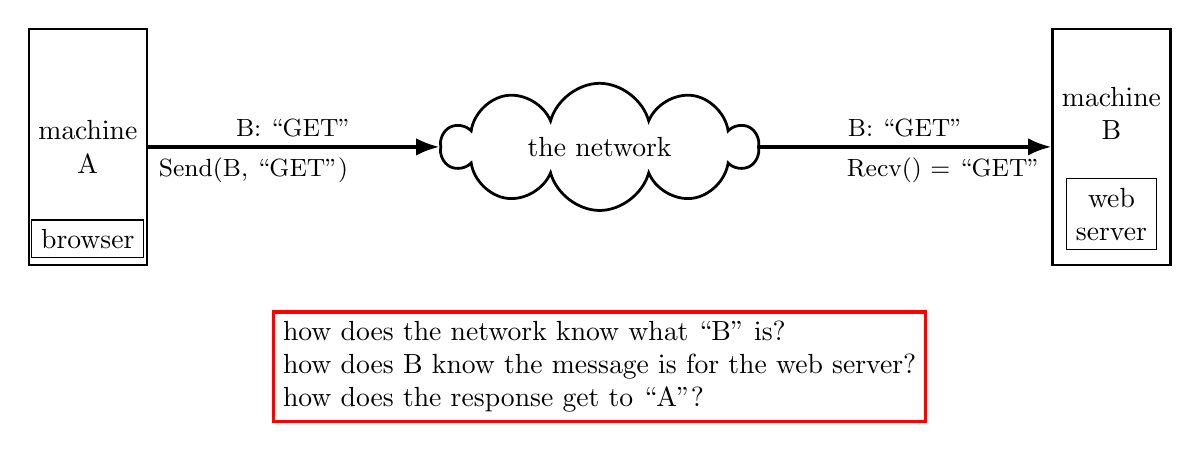
\begin{tikzpicture}
    \tikzset{
        >=Latex,
        comp box/.style={draw, thick, align=center, minimum width=1.5cm,minimum height=3cm},
        explain box/.style={draw=red,very thick, align=left},
        msg/.style={font=\small},
        cmd/.style={font=\small},
    }
        \node[comp box] (machine A) at (-6.5, 0) {machine \\ A};
        \node[draw,cloud,line width=1pt,minimum width=4cm,minimum height=1cm,aspect=3,
                ] (network) at (0,0) {the network};
        \node[comp box] (machine B) at (6.5, 0) {machine \\ B\\ ~\\~};
        \draw[very thick,->] (machine A) -- (network)
            node[midway,above,msg] {B: ``GET''}
            node[pos=0.0,below right,cmd] {Send(B, ``GET'')};
        \draw[very thick,<-] (machine B) -- (network)
            node[midway,above,msg] {B: ``GET''}
            node[pos=0.0,below left,cmd] {Recv() = ``GET''};
        % FIXME: hilite network: knows how to get message to particular place
            % note/show buffering at A/B


        \node[anchor=south,draw,rectangle,] at ([yshift=.1cm]machine A.south) {
            browser
        };
        \node[explain box,anchor=north] at ([yshift=-1.25cm]network.south) {
            how does the network know what ``B'' is? \\
            how does B know the message is for the web server? \\
            how does the response get to ``A''?
        };
        \node[anchor=south,draw,rectangle,align=center] at ([yshift=.2cm]machine B.south) {
            web\\server
        };
    \end{tikzpicture}
\end{frame}

\usetikzlibrary{arrows.meta,calc,positioning,shapes.callouts,shapes.symbols}

\begin{frame}[label=nameAndAddr]{names and addresses}
\small
\begin{tabular}{l|l}
\textbf{name} & \textbf{address} \\\hline
\large\myemph{logical identifier} & \large\myemph{location/how to locate} \\
~ & ~ \\
variable \texttt{counter} & memory address \texttt{0x7FFF9430} \\ 
~ & ~ \\
DNS name \texttt{www.virginia.edu} & IPv4 address \texttt{128.143.22.36} \\
DNS name \texttt{mail.google.com} & IPv4 address \texttt{216.58.217.69} \\
DNS name \texttt{mail.google.com} & IPv6 address \fontsize{10}{11}\selectfont\texttt{2607:f8b0:4004:80b::2005} \\
    DNS name \fontsize{9.5}{10.5}\selectfont\texttt{reiss-t3620.cs.virginia.edu} & IPv4 address \texttt{128.143.67.91} \\
    DNS name \fontsize{9.5}{10.5}\selectfont\texttt{reiss-t3620.cs.virginia.edu} & MAC address \texttt{18:66:da:2e:7f:da} \\
~ & ~ \\
service name \texttt{https} & port number \texttt{443} \\
service name \texttt{ssh} & port number \texttt{22} \\
\end{tabular}
\end{frame}



% \section{a frame example}
% \againframe<4>{layerOverview}
% \input{../network/example-frame}



\section{IP}
% FIXME: example sending message multiple hop
\againframe<5>{layerOverview}
\usetikzlibrary{calc,positioning,shapes.callouts}

\begin{frame}{the network layer}
\begin{itemize}
\item the Internet Protocool (IP) version 4 or version 6
    \begin{itemize}
    \item there are also others, but quite uncommon today
    \end{itemize}
\item allows send messages to/recv messages from other networks
    \begin{itemize}
    \item ``internetwork''
    \end{itemize}
\item messages usually called ``packets''
\end{itemize}
\end{frame}


\subsection{IPv4 addresses}
\input{../network/ipv4}

\subsection{IPv6 addresses}
\input{../network/ipv6}

\subsection{routing idea}

\begin{frame}{IPv4 addresses and routing tables}
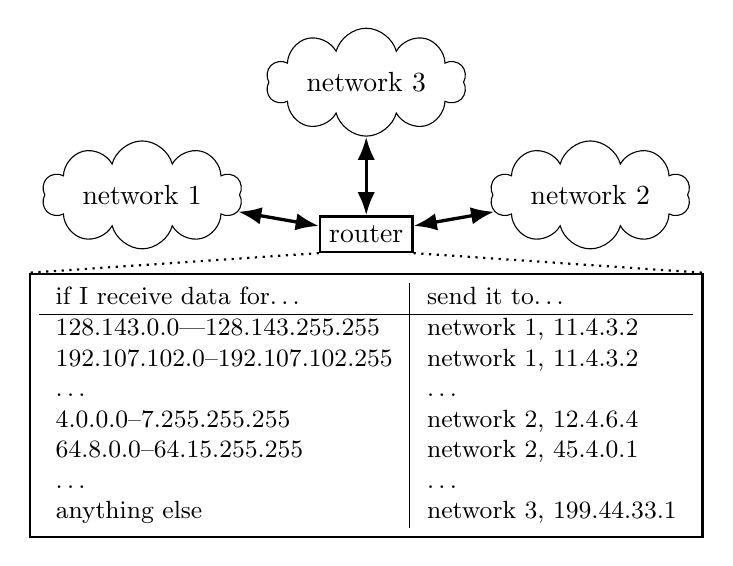
\begin{tikzpicture}
\tikzset{>=Latex},
\node[draw,thick] (router) {router};
\node[aspect=3,draw,cloud,anchor=east,minimum width=2.5cm] (network 1) at ([xshift=-1cm,yshift=.5cm] router.west) {
    network 1
};
\node[aspect=3,draw,cloud,anchor=west,minimum width=2.5cm] (network 2) at ([xshift=1cm,yshift=.5cm] router.east) {
    network 2
};
\node[aspect=3,draw,cloud,anchor=south,minimum width=2.5cm] (network 3) at ([yshift=1cm] router.north) {
    network 3
};
\foreach \x in {1,2,3} { \draw[<->,very thick] (router) -- (network \x); }
\node[anchor=north,font=\small,draw,thick] (table) at ([yshift=-.25cm]router.south) {
\begin{tabular}{l|l}
if I receive data for\ldots & send it to\ldots \\ \hline
128.143.0.0---128.143.255.255 & network 1, 11.4.3.2 \\
192.107.102.0--192.107.102.255 & network 1, 11.4.3.2 \\
\ldots & \ldots \\
4.0.0.0--7.255.255.255 & network 2, 12.4.6.4 \\
64.8.0.0--64.15.255.255 & network 2, 45.4.0.1  \\
\ldots & \ldots \\
anything else & network 3, 199.44.33.1 \\
\end{tabular}
};
\draw[thick,dotted] (router.south west) -- (table.north west);
\draw[thick,dotted] (router.south east) -- (table.north east);
\end{tikzpicture}
\end{frame}




% \subsection{special addresses}
% \begin{frame}{selected special IPv4 addresses}
\begin{itemize}
\item 127.0.0.0 --- 127.255.255.255 --- localhost
    \begin{itemize}
    \item AKA loopback
    \item the machine we're on
    \item typically only 127.0.0.1 is used
    \end{itemize}
\item 192.168.0.0--192.168.255.255 and \\ 10.0.0.0--10.255.255.255 and \\ 172.16.0.0--172.31.255.255 
    \begin{itemize}
    \item ``private'' IP addresses
    \item not used on the Internet
    \item commonly connected to Internet with \myemph{network address translation}
    \item also 100.64.0.0--100.127.255.255 (but with restrictions)
    \end{itemize}
\item 169.254.0.0-169.254.255.255
    \begin{itemize}
    \item link-local addresses --- `never' forwarded by routers
    \end{itemize}
\end{itemize}
\end{frame}

\begin{frame}{network address translation}
\begin{itemize}
\item IPv4 addresses are kinda scarce
\item solution: \textit{convert} many private addrs. to one public addr.
\item locally: use private IP addresses for machines
\item outside: private IP addresses become a single public one
\item commonly how home networks work (and some ISPs)
\end{itemize}
\end{frame}


\section{TCP/UDP}
\againframe<6>{layerOverview}

\subsection{port numbers}
\begin{frame}{port numbers}
    \begin{itemize}
    \item we run multiple programs on a machine
        \begin{itemize}
        \item IP addresses identifying machine --- not enough
        \end{itemize}
    \item<2-> so, add 16-bit \textit{port numbers}
        \begin{itemize}
        \item<2-> think: multiple PO boxes at address
        \end{itemize}
    \vspace{.5cm}
    \item<3-> 0--49151: typically assigned for particular services
        \begin{itemize}
        \item 80 = http, 443 = https, 22 = ssh, \ldots
        \end{itemize}
    \item<3-> 49152--65535: allocated on demand
        \begin{itemize}
        \item default ``return address'' for client connecting to server
        \end{itemize}
    \end{itemize}
\end{frame}





\subsection{OS tracking connections}
% \begin{frame}{connections in TCP/IP}
    \begin{itemize}
    \item connection identified by \textit{5-tuple}
        \begin{itemize}
        \item used by OS to lookup ``where is the socket?''
        \end{itemize}
    \item \small(protocol=TCP/UDP, local IP addr., local port, remote IP addr., remote port)
    \vspace{.5cm}
    \item local IP address, port number can be set with \texttt{bind()} function
        \begin{itemize}
        \item \textit{typically} always done for servers, not done for clients
        \item system will choose default if you don't
        \end{itemize}
    \end{itemize}
\end{frame}

\begin{frame}[fragile,label=laptopNetstat]{connections on my desktop}
\begin{lstlisting}[language={},basicstyle=\fontsize{9.5}{10.5}\selectfont]
cr4bd@reiss-t3620>/u/cr4bd
$ netstat --inet --inet6 --numeric
Active Internet connections (w/o servers)
Proto Recv-Q Send-Q Local Address           Foreign Address         State      
tcp        0      0 128.143.67.91:49202     128.143.63.34:22        ESTABLISHED
tcp        0      0 128.143.67.91:803       128.143.67.236:2049     ESTABLISHED
tcp        0      0 128.143.67.91:50292     128.143.67.226:22       TIME_WAIT  
tcp        0      0 128.143.67.91:54722     128.143.67.236:2049     TIME_WAIT  
tcp        0      0 128.143.67.91:52002     128.143.67.236:111      TIME_WAIT  
tcp        0      0 128.143.67.91:732       128.143.67.236:63439    TIME_WAIT  
tcp        0      0 128.143.67.91:40664     128.143.67.236:2049     TIME_WAIT  
tcp        0      0 128.143.67.91:54098     128.143.67.236:111      TIME_WAIT  
tcp        0      0 128.143.67.91:49302     128.143.67.236:63439    TIME_WAIT  
tcp        0      0 128.143.67.91:50236     128.143.67.236:111      TIME_WAIT  
tcp        0      0 128.143.67.91:22        172.27.98.20:49566      ESTABLISHED
tcp        0      0 128.143.67.91:51000     128.143.67.236:111      TIME_WAIT  
tcp        0      0 127.0.0.1:50438         127.0.0.1:631           ESTABLISHED
tcp        0      0 127.0.0.1:631           127.0.0.1:50438         ESTABLISHED
\end{lstlisting}
\end{frame}

\begin{frame}{non-connection sockets}
\begin{itemize}
\item TCP servers waiting for connections + \\
UDP sockets with no particular remote host
\item Linux: OS keeps 5-tuple with ``wildcard'' remote address
\end{itemize}
\end{frame}

\begin{frame}[fragile,label=laptopNetstat]{``listening'' sockets on my desktop}
\begin{lstlisting}[language={},basicstyle=\fontsize{9.5}{10.5}\selectfont]
cr4bd@reiss-t3620>/u/cr4bd
$ netstat --inet --inet6 --numeric --listen
Active Internet connections (only servers)
Proto Recv-Q Send-Q Local Address           Foreign Address         State      
tcp        0      0 127.0.0.1:38537         0.0.0.0:*               LISTEN     
tcp        0      0 127.0.0.1:36777         0.0.0.0:*               LISTEN     
tcp        0      0 0.0.0.0:41099           0.0.0.0:*               LISTEN     
tcp        0      0 0.0.0.0:45291           0.0.0.0:*               LISTEN     
tcp        0      0 127.0.0.1:51949         0.0.0.0:*               LISTEN     
tcp        0      0 127.0.0.1:41071         0.0.0.0:*               LISTEN     
tcp        0      0 0.0.0.0:111             0.0.0.0:*               LISTEN     
tcp        0      0 127.0.0.1:32881         0.0.0.0:*               LISTEN     
tcp        0      0 127.0.0.1:38673         0.0.0.0:*               LISTEN     
....
tcp6       0      0 :::42689                :::*                    LISTEN
udp        0      0 128.143.67.91:60001     0.0.0.0:*
udp        0      0 128.143.67.91:60002     0.0.0.0:*
...
udp6       0      0 :::59938                :::* 
\end{lstlisting}
\end{frame}

\begin{frame}{connections in TCP/IP}
    \begin{itemize}
    \item connection identified by \textit{4-tuple}
        \begin{itemize}
        \item used by OS to lookup ``where is the socket?''
        \end{itemize}
    \item \small(local IP address, local port, remote IP address, remote port)
    \vspace{.5cm}
    \item local IP address, port number can be set with \texttt{bind()} function
        \begin{itemize}
        \item \textit{typically} always done for servers, not done for clients
        \item system will choose default if you don't
        \end{itemize}
    \end{itemize}
\end{frame}

\section{DNS}
\againframe<2>{nameAndAddr}
\input{../network/dns}

\subsection{URLs and URIs}
\input{../network/urls}

\subsection{HTTP}
\begin{frame}[fragile]{HTTP: HyperText Transfer Protocol}
\begin{itemize}
    \item primary application-layer protocol for the Web
    \item standard port: 80 (non-encrypted), 443 (encrypted)
    \item uses TCP (or TCP + TLS for encrypted version)
    \item client-server protocol
        \begin{itemize}
        \item server = always on machine, never initiaites contact
        \item client = sometimes on machine, initiates contact
        \end{itemize}
    \item ex. URL: \texttt{http://www.foo.com/bar}
\end{itemize}
\end{frame}

\begin{FragileFrame}
\frametitle{HTTP: HyperText Transfer Protocol}
\begin{itemize}
    \item \texttt{http://www.foo.com/bar}
    \item HTTP client (example: web browser) connects to www.foo.com
    \item sends something like
\end{itemize}
\begin{Verbatim}
GET /bar HTTP/1.1
Host: www.foo.com
...
\end{Verbatim}
    \begin{itemize}
    \item server replies with status code + (usually) some data
        \begin{itemize}
        \item 200 OK, 403 Unauthorized 404 Not Found, 500 Internal Server Error, \ldots
        \end{itemize}
    \end{itemize}
\end{FragileFrame}

\begin{FragileFrame}
    \frametitle{HTTP miscellany}
    \begin{itemize}
        \item other HTTP commands besides GET
        \item POST --- sending forms
        \item HEAD --- get metadata about file (without getting its data)
        \item PUT, DELETE, \ldots 
        \vspace{.5cm}
        \item all requests/replies have many possible headers
            \begin{itemize}
            \item filetype inforation
            \item login-related information (usually)
            \item metadata used for caching webpages
            \item \ldots
            \end{itemize}
    \end{itemize}
\end{FragileFrame}



% \section{DHCP and IPv6 autoconfig}
% 
\begin{frame}{autoconfiguration}
\begin{itemize}
\item problem: how does my machine get IP address
\vspace{.5cm}
\item otherwise:
    \begin{itemize}
    \item have sysadmin type one in?
    \item just choose one?
    \item \myemph<2>{ask someone on local network to assign it}
    \end{itemize}
\end{itemize}
\end{frame}

\begin{frame}{DHCP high-level}
    \begin{itemize}
    \item protocol done over UDP
    \vspace{.5cm}
    \item but since we don't have IP address yet, use \texttt{0.0.0.0}
    \item and since we don't know server address, use \texttt{255.255.255.255}
        \begin{itemize}
        \item = ``everyone on the local network''
        \end{itemize}
    \item local server replies to request with address + time limit
    \end{itemize}
\end{frame}



\section{NAT}
\begin{frame}{network address translation}
\begin{itemize}
\item IPv4 addresses are kinda scarce
\item solution: \textit{convert} many private addrs. to one public addr.
\item locally: use private IP addresses for machines
\item outside: private IP addresses become a single public one
\item commonly how home networks work (and some ISPs)
\end{itemize}
\end{frame}

\begin{frame}{implementing NAT}
\small
\begin{tabular}{llll}
remote host + port & outside local port number & inside IP & inside port number \\ \hline
128.148.17.3:443 & 54033 & 192.168.1.5 & 43222 \\
11.7.17.3:443 & 53037 & 192.168.1.5 & 33212 \\
128.148.31.2:22 & 54032 & 192.168.1.37 & 43010 \\
128.148.17.3:443 & 63039 & 192.168.1.37 & 32132 \\
\end{tabular}
\begin{itemize}
\item table of the translations
\item need to update as new connections made
\end{itemize}
\end{frame}

\begin{frame}{NAT and layers}
    \begin{itemize}
    \item previously: network layer responsible for get to right machine
    \item now: network + transport layer
        \begin{itemize}
        \item because we use port numbers
        \end{itemize}
    \item also, NAT needs to know about connections (transport layer)
        \begin{itemize}
        \item to know how to setup/remove table entries
        \end{itemize}
    \end{itemize}
\end{frame}


\section{lab API}
\begin{frame}{upcoming lab}
    \begin{itemize}
    \item request + receive message split into pieces
    \item you are responsible for:
        \begin{itemize}
        \item requesting parts in order
        \item \myemph<2>{resending requests if messages lost/corrupted}
        \end{itemize}
    \item \myemph<2>{``acknowledge'' receiving part X to request part X+1}
    \end{itemize}
\end{frame}

\begin{frame}{protocol}
    \begin{itemize}
    \item {\tt GET$x$} --- retrieve message $x$ (x = 0, 1, 2, or 3)
        \begin{itemize}
        \item other end acknowledges by giving data
        \item if they don't reply, you need to send again
        \item higher numbered messages have errors/etc. that are harder to handle
        \end{itemize}
    \item {\tt ACK$n$ }
        \begin{itemize}
        \item request message $n + 1$ by acknowledging message $n$
        \item not quite same purpose as acknowledgments in prior examples
        \item \myemph<2>{(in lab, the response is your `acknowledgment' of your request;} \\
            \myemph<2>{you retry if you don't get it)}
        \end{itemize}
    \end{itemize}
\end{frame}


\begin{frame}[fragile]{callback-based programming (1)}
\begin{Verbatim}[fontsize=\small]
/* library code you don't write */
/* in the lab: part of waitForAllTimeoutsAndMessagesThenExit() */
void mainLoop() {
    while (notExiting) {
        Event event = waitForAndGetNextEvent();
        if (event.type == RECIEVED) {
            recvd(...);
        } else if (event.type == TIMEOUT) {
            (event.timeout_function)(...);
        }
        ...
    }
}
\end{Verbatim}
\end{frame}

\begin{frame}[fragile]{callback-based programming (2)}
\begin{Verbatim}[fontsize=\small]
/* your code, called by library */
void recvd(...) {
    ...
    setTimeout(..., timerCallback, ...);
}

void timerCallback(...) {
    ...
}

int main() {
    send(.../* first message */);
    ... /* other initial setup */
    waitForAllTimeoutsAndMessagesThenExit(); // runs mainLoop()
}
\end{Verbatim}
\end{frame}


\begin{frame}{callback-based programming}
    \begin{itemize}
    \item writing scripts in a webpage
    \item many graphical user interface libraries
    \item sometimes servers that handle lots of connections
    \end{itemize}
\end{frame}

